% !Mode:: "TeX:UTF-8"
%% 请使用 XeLaTeX 编译本文.
\documentclass{HEBUTMaster}   % 选项 forprint: 交付打印时, 建议加上此选项, 以消除彩色链接文字, 避免彩色字迹打印偏淡.
                              % 选项 forlib: 提交给图书馆的电子版, 需要加上选项 forlib, 以消除空白页和彩色链接.
                              % 选项 smd: Specialist Master's Degree, 产生专业硕士学位论文封面、页眉.
%===============================================参考文献=====================================================%
\bibliographystyle{abbrv}        % 参考文献样式,  plain,unsrt,alpha,abbrv 等等

%===============================================  正文  =====================================================%
\begin{document} 

%===============================================  信息  =====================================================%
\title{基于机器学习的缺陷图像数据集处理

课程报告}
\Etitle{Defect image data set processing based on machine learning

Course Report} % 英文题目

\author{程淑伟}
\StudentNumber{202032803115}  % 学号
\Eauthor{Cheng Shuwei}  %作者英文名

\Csupervisor{石陆魁\quad 教授}  %指导教师中文名、职称
\Esupervisor{Prof.~Shi Lukui}  %指导教师英文名、职称

\Schoolname{School of Artificial Intelligence} %学院英文名. 不确定的话, 请看一下自己学院的网页上是怎么写的. 别搞错了!

\date{二〇二一年四月} % 硕士类只写年月. 要注意和英文日期一致!!
\Edate{Apr, 2020} % 英文封面日期

%%%=====================================================================%%%
\pdfbookmark[0]{封面}{title}         % 封面页加到 pdf 书签
\maketitle
%%%=====================================================================%%%
% !Mode:: "TeX:UTF-8"

%%% 此部分包含: (1) 英文封面 (无需改动) ; (2) 郑重声明 (无需改动).

%%%%%%%%%%%%%%%%%%%%%%%%%%%%%
%%% -------------  英文封面 (无需改动)-------------   %%%
%%%%%%%%%%%%%%%%%%%%%%%%%%%%%
\thispagestyle{empty}
\renewcommand{\baselinestretch}{1.5}  %下文的行距
\vspace*{0.5cm}

\begin{center}{\zihao{2} \the\Etitle \par}\end{center}

\vfill

\begin{center}
\zihao{4}
\begin{tabular}{ r l }
 Candidate:      &  {\sc \the\Eauthor}      \\
 Student Number: & {\the\StudentNumber} \\
 Supervisor:     &  {\sc \the\Esupervisor}   \\
 Major:          & \the\Emajor  \\
\ifsmd \else Speciality:     & \the\Especiality \fi
\end{tabular}

\vspace*{2cm}
\begin{center}
  \iflib % 向图书馆提交电子文档, 使用黑白校徽.
  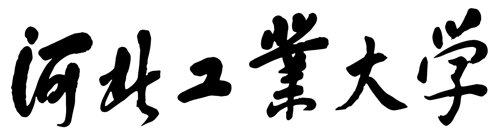
\includegraphics[height=4cm]{hebut.png}       %%  黑白的. 很小, 只有 10k.
  \else
     \ifprint % 文档打印, 使用黑白校徽.
  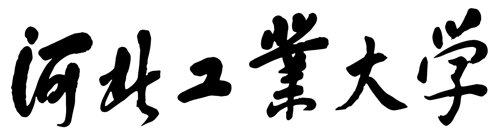
\includegraphics[height=4cm]{hebut.png}       %%  黑白的.
  \else
  
\includegraphics[height=4cm]{hebut1.png} %%  彩色的.
  \fi
  \fi
\end{center}


\zihao{-2}
\the\Schoolname\\
{\sc Hebei University of Technology}

\vspace*{1.0cm}

\the\Edate

\end{center}
%%%%%%%--判断是否需要空白页-----------------------------
 \iflib
 \else
\newpage
\thispagestyle{empty}
 \cleardoublepage
 \fi
%%%%%%%-------------------------------------------------
%%%--- 加入``郑重声明'' --- %%%%%%%%%%%%%%%%%
{\pagestyle{empty}
\newpage
\vspace*{20pt}
\begin{center}{\ziju{0.8}\zihao{-2}\heiti 论文原创性声明}\end{center}
\par\vspace*{30pt}
\renewcommand{\baselinestretch}{2}
{\zihao{4} \songti %


本人郑重声明: 所呈交的论文, 是本人独立进行研究工作所取得的研究成果.
除文中已经标明引用的内容外, 本论文不包含任何其他个人或集体已经发表或撰写过的研究成果.
对本文的研究做出贡献的个人和集体, 均已在文中以明确方式标明. 本声明的法律结果由本人承担.


\vskip2cm

\hspace*{4cm}学位论文作者(签名): \hspace{4cm} \hfill \\[1cm]
\hspace*{10cm}年 \hfill  月 \hfill 日\hspace{1cm}\hfill\par}

%%%%%%%--判断是否需要空白页-----------------------------
  \iflib
  \else
  \newpage
  \cleardoublepage
  \fi
%%%%%%%-------------------------------------------------
}
\renewcommand{\baselinestretch}{1.6}
\small\normalsize




    % 加入英文封面
\frontmatter
\pagenumbering{Roman}               % 正文之前的页码用大写罗马字母编号.

\cleardoublepage
\newpage  \pagestyle{fancy} \fancyfancy
%%%=====================================================================%%%
% !Mode:: "TeX:UTF-8"

%%% 说明: 此部分需要自己填写的内容:  (1) 中文摘要及关键词 (2) 英文摘要及关键词

%%%%%%%%%%%%%%%%%%%%%%%
%%% ------------ 中文摘要 ---------------%%%
%%%%%%%%%%%%%%%%%%%%%%%
\begin{cnabstract}


\end{cnabstract}
\vspace{1em}\par\vfill

%%%--------- 关键词 -------- %%%
\cnkeywords{}

%%%%%%%%%%%%%%%%%%%%%%%


%%%%%%%%%%%%%%%%%%%%%%%
%%% ------------ 英文摘要 ---------------%%%
%%%%%%%%%%%%%%%%%%%%%%%

\begin{enabstract}





\end{enabstract}
\vspace{1em}\par\vfill

%%%------ 英文关键词 ------- %%%
\enkeywords{}


      % 加入中英文 摘要 .
%---把目录加入到书签---%%%%%%%%%%%%%%
\pdfbookmark[0]{目录}{toc}%%%%%%%%%%%%

\tableofcontents
%%%=====================================================================%%%
\mainmatter %% 以下是正文
\baselineskip=20pt  % 正文行距为 20 磅


%%%================================第一章=====================================%%%
\chapter{课程作业简介}

该数据集包括4类样本,完成下列任务:
\begin{enumerate}[(1)]
  \item  利用PCA对数据降维,可视化2、3结果,不同类用不同的颜色表示。
  \item  提取特征,至少提取两种图像特征。
  \item  在提取的特征上比较SVM、BP神经网络、随机森林分类的结果。
  \item  撰写课程报告:包括数据集描述、PCA介绍、特征提取方法介绍、分类模型介绍、1-3中实验结果,实验结果讨论
\end{enumerate}


%%%================================第二章=====================================%%%
\chapter{数据集描述}
%%%================================第2.1章=====================================%%%


%%%================================第二章=====================================%%%
\chapter{PCA介绍}
在多元统计分析中,主成分分析(英语:Principal components analysis,PCA)是一种统计分析、简化数据集的方法。它利用正交变换来对一系列可能相关的变量的观测值进行线性变换,从而投影为一系列线性不相关变量的值,这些不相关变量称为主成分(Principal Components)。具体地,主成分可以看做一个线性方程,其包含一系列线性系数来指示投影方向。PCA对原始数据的正则化或预处理敏感(相对缩放)。

\section{基本思想}
\begin{itemize}
  \item  将坐标轴中心移到数据的中心,然后旋转坐标轴,使得数据在C1轴上的方差最大,即全部n个数据个体在该方向上的投影最为分散。意味着更多的信息被保留下来。C1成为第一主成分。
  \item 第二主成分:找一个C2,使得C2与C1的协方差(相关系数)为0,以免与C1信息重叠,并且使数据在该方向的方差尽量最大。
  \item  以此类推,找到第三主成分,第四主成分……第p个主成分。p个随机变量可以有p个主成分。
\end{itemize}

主成分分析经常用于减少数据集的维数,同时保留数据集当中对方差贡献最大的特征。这是通过保留低维主成分,忽略高维主成分做到的。这样低维成分往往能够保留住数据的最重要部分。但是,这也不是一定的,要视具体应用而定。由于主成分分析依赖所给数据,所以数据的准确性对分析结果影响很大。

主成分分析由卡尔·皮尔逊于1901年发明,用于分析数据及建立数理模型,在原理上与主轴定理相似。之后在1930年左右由哈罗德·霍特林独立发展并命名。依据应用领域的不同,在信号处理中它也叫做离散K-L 转换(discrete Karhunen–Loève transform (KLT))。其方法主要是通过对协方差矩阵进行特征分解,以得出数据的主成分(即特征向量)与它们的权值(即特征值)。PCA是最简单的以特征量分析多元统计分布的方法。其结果可以理解为对原数据中的方差做出解释:哪一个方向上的数据值对方差的影响最大?换而言之,PCA提供了一种降低数据维度的有效办法;如果分析者在原数据中除掉最小的特征值所对应的成分,那么所得的低维度数据必定是最優化的(也即,这样降低维度必定是失去信息最少的方法)。主成分分析在分析复杂数据时尤为有用,比如人脸识别。

PCA是最简单的以特征量分析多元统计分布的方法。通常,这种运算可以被看作是揭露数据的内部结构,从而更好地展现数据的变异度。如果一个多元数据集是用高维数据空间之坐标系来表示的,那么PCA能提供一幅较低维度的图像,相当于数据集在讯息量最多之角度上的一个投影。这样就可以利用少量的主成分让数据的维度降低了。
PCA 跟因子分析密切相关。因子分析通常包含更多特定领域底层结构的假设,并且求解稍微不同矩阵的特征向量。
PCA 也跟典型相关分析(CCA)有关。CCA定义的坐标系可以最佳地描述两个数据集之间的互协方差,而PCA定义了新的正交坐标系,能最佳地描述单个数据集当中的方差。

%%%================================第三章=====================================%%%
\chapter{特征提取}
特征提取(英语:Feature extraction)在机器学习、模式识别和图像处理中有很多的应用。特征提取是从一个初始测量的资料集合中开始做,然后建构出富含资讯性而且不冗余的导出值,称为特征值(feature)。它可以帮助接续的学习过程和归纳的步骤,在某些情况下可以让人更容易对资料做出较好的诠释。特征提取是一个降低维度的步骤,初始的资料集合被降到更容易管理的族群(特征)以便于学习,同时保持描述原始资料集的精准性与完整性。

当一个算法的输入资料太过于庞大冗余以至于不便处理(如:一样的测量方法但是分别使用英尺和米表示,或是影像中像素的重复性),这些资料可以被转换成化简后的特征集合,也称作特征向量(feature vector),决定这些原始资料子集的步骤称为特征提取。成功的情形下,被选择的特征包含跟输入资料相关的资讯,因此这些被化简后的特征能够被用来做理想的任务,而不使用原始完整的初始资料来做这个任务。

\section{概论}
相较于原始庞大的资料集合需要很大量的资源来描述,特征提取可以减少需要描述这些资料的资源。当我们分析复杂资料时,其中一个主要的问题是源自于变数的数量过多。分析很多个变数一般来说需要很大量的内存以及计算能力,同时太多变数也可能造成分类问题的算法有过度拟合于训练资料的现象,因此对新的采样无法有效地归纳。特征提取是处理变数组合并维持资料充足的准确性时,常通称的术语。很多机器学习的实作者认为适当的特征提取是有效模型构建的关键。

可以利用已经建构好的应用相关的特征集合来改善结果,通常这样的特征集合是被专家所建构。其中一种此类处理被叫做特征工程师。除此之外,我们也可以使用一般的降维技术,如下:
\begin{itemize}
  \item 独立成分分析
  \item 等距特征映射
  \item 核主成分分析
  \item 潜在语义学
  \item 偏最小二乘回归
  \item 主成分分析
  \item 多因子降维法
  \item 非线性降维
  \item 多线性主成分分析
  \item 半定式嵌入
  \item 自编码器
\end{itemize}

\section{特征类型}
\begin{itemize}
  \item 边缘

边缘是组成两个图像区域之间边界(或边缘)的像素。一般一个边缘的形状可以是任意的,还可能包括交叉点。在实践中边缘一般被定义为图像中拥有大的梯度的点组成的子集。一些常用的算法还会把梯度高的点联系起来来构成一个更完善的边缘的描写。这些算法也可能对边缘提出一些限制。
局部地看边缘是一维结构。
  \item 角

角是图像中点似的特征,在局部它有两维结构。早期的算法首先进行边缘检测,然后分析边缘的走向来寻找边缘突然转向(角)。后来发展的算法不再需要边缘检测这个步骤,而是可以直接在图像梯度中寻找高度曲率。后来发现这样有时可以在图像中本来没有角的地方发现具有同角一样的特征的区域。
\item 区域

与角不同的是区域描写一个图像中的一个区域性的结构,但是区域也可能仅由一个像素组成,因此许多区域检测也可以用来检测角。一个区域监测器检测图像中一个对于角监测器来说太平滑的区域。
区域检测可以被想象为把一张图像缩小,然后在缩小的图像上进行角检测。
  \item 脊

长条形的物体被称为脊。在实践中脊可以被看作是代表对称轴的一维曲线,此外局部针对于每个脊像素有一个脊宽度。从灰梯度图像中提取脊要比提取边缘、角和区域困难。在空中摄影中往往使用脊检测来分辨道路,在医学图像中它被用来分辨血管。
\end{itemize}
%%%================================第四章=====================================%%%
\chapter{分类模型介绍}
\section{朴素贝叶斯}
应用:简单,容易理解的一种分类算法,常用于文本分类、垃圾邮件处理,属于监督学习。

原理:基于贝叶斯定理,对于给出的待分类项,求解在待分类项出现的条件下各个类别的概率;也就是已知先验概率,求解在某一条件发生下的后验概率。当出现某一后验项概率为0时,就是说某类别下某个特征没有出现,需要使用Laplace校准。

输入与输出:输入为某个类别发生的概率(先验概率)和某类别下出现某个特征的概率,输出为某特征划分为某个类别的概率(后验概率),根据概率的大小判断是否属于这个类别。

优势劣势:理解、计算简单,易于实现。对小规模数据表现很好,对于大量规模数据表现欠佳,算法朴素地认为各特征之间相互独立、没有影响,因此在处理相关性较大的特征时,表现不好

\section{逻辑回归}
应用:主要用于离散变量的分类——属于监督学习的一种;一个单独的逻辑回归只能判别两个类——二分类回归,通过一个概率值判断属于哪一个分类。

原理:模型通过定义一个sigmoid S型预测函数,取值范围(0,1)预测不同的分类结果,默认阈值0.5,大于0.5则认为属于分类1,小于0.5认为属于分类2。通过代价函数(cost function)评估预测函数的好坏——使用梯度下降算法能够找到损失函数最小值。

输入与输出:输入一个线性组合,也就是一个带权重的特征组合(自变量),输出结果表征了某个样本属于某类别的概率(即可能性,取值0~1)。

优势劣势:朴素贝叶斯(生成模型)将不同特征处理成为独立不相关的变量,会有一定误差,逻辑回归(判别模型)不管各特征之间是否有联系,可以直接将任何特征组合扔进模型;朴素贝叶斯处理数据规模较小的集合,对于大量数据,逻辑回归更有优势;逻辑回归容易过拟合,分类精度不太高。

解决方案:1)减少特征数量(减少特征会失去一些信息,即使特征选的很好)人工选择要保留的特征。2)正则化(特征较多时比较有效)

\section{决策树}
应用:通过训练数据,进行分类。也可以用来作回归。

原理:一种描述对实例分类的树结构,两种节点:内部节点和叶子结点——内部节点表示一个特征或属性,叶子结点表示一个分类。将特征看作一个内部节点,对每个内部节点进行递归分割(两种分割方式:连续性——用>=,<分割,离散型——按类别分割),递归停止条件:每个叶子节点只有一个类型,或者设置节点记录数量低于一个设定的阈值。根据纯度来构建决策树,纯度指节点分割后有最小的分类(例子:“拥有房产”,可以将记录分成了两类,“是”的节点全部都可以偿还债务,非常“纯”,“否”的分支再继续下一个节点分割)。不纯度量化:ID3算法使用信息增益(纯度差)、C4.5算法使用信息增益率、CART算法使用基尼系数,取值越小,不纯度越低,纯度越高,节点更靠近根节点。

决策树步骤:特征选择-决策树生成-剪枝。

优势劣势:容易理解,效率高;可以处理连续型和离散变量,通过不纯度来分割变量;容易过拟合

解决方案:1)裁剪枝叶;2)随机森林

\section{随机森林}
应用:由于决策树可能出现的误差和过拟合问题,使用RF可更好地解决分类和回归问题。

原理:RF算法是将决策树进行Bagging,使用多棵树进行单独预测,最后将这些预测进行组合决定。通常多个弱分类器通过组合可以得到很强的决策效果。

保证每棵树之间的独立性,采用3层随机性:

1、每棵树的数据有放回随机抽样;

2、每棵树的特征也随机抽取,数量通常为sqrt(N)或者log2(N)+1;

3、多个特征进行分割时,随机选择一个进行分割。

优势劣势:解决了过拟合问题,增加稳定性,提升预测精度;可以对数据降维,只选取少量几个重要特征来近似表示原数据——用于特征选择,选择关键特征;可并行,能处理大规模数据;模型过大,需要存储空间大,模型加载时间长;噪声比较大的样本,容易过拟合

\section{SVM}
应用:可以应用于分类和回归,分类模型通常用做二分类。

原理:基于逻辑回归线性分类,定义在特征空间上的间隔最大的线性分类器,利用间隔最大化求最优分离超平面。定义一个超平面方程,使得其到不同分类数据点的距离最大,即为最优超平面(如图中的实线wTx+b=0)。大多数情况下,数据并不是线性可分的,使用核函数(Kernel)。

核函数思想——由于线性不可分,将数据集映射到高维,变成线性可分。将数据在低维计算,将分类效果表现在高维。

优势劣势:可用于分类和回归;容易解释;计算复杂度低;可以处理小样本,非线性问题;通过处理低维度数据解决高维度问题;原始SVM只擅长解决二分类问题

%%%================================第五章=====================================%%%
\chapter{1-3中实验结果}

%%%================================第六章=====================================%%%
\chapter{实验结果讨论}










%%%================================参考文献=====================================%%%
\cleardoublepage\phantomsection
\addcontentsline{toc}{chapter}{参考文献}
\begin{thebibliography}{000}\zihao{5}

  \bibitem{r1} https://my.oschina.net/nekyo/blog/1594113
  \bibitem{r2} https://mathpretty.com/10998.html#%E4%BD%BF%E7%94%A8PCA%E9%99%8D%E7%BB%B4
  \bibitem{r3}
  \bibitem{r4}
  \bibitem{r5}  
  \bibitem{r6} 
  
\end{thebibliography}


\acknowledgement
感谢曹斌老师布置的作业, 加快了我科研的脚步,感谢!

%\backmatter
%% !Mode:: "TeX:UTF-8"

%%% 此部分内容:  (1) 致谢  (2) 河北工业大学学位论文使用授权协议书(无需改动)

%%%%%%%%%%%%%%%%%%%%%%%
%%% --------------- 致谢 ------------- - %%%
%%%%%%%%%%%%%%%%%%%%%%%
\acknowledgement


感谢你, 感谢他和她, 感谢大家.







%%%%%---河北工业大学学位论文使用授权协议书---%%%%%%%%%%%%
%%%%%%%%%%%%%%%%%%%%%%%%%%%%%%%%%%%
%%%%%%%%%%%%%%%%%%%%%%%%%%%%%%%%%%%
\cleardoublepage
\newpage\vspace*{20pt}
\begin{center}{\zihao{-2}\heiti 河北工业大学学位论文使用授权协议书}\end{center}
\par\vspace*{30pt}

本论文作者愿意遵守河北工业大学关于保存、使用学位论文的管理办法及规定,
即:学校有权保存学位论文的印刷本和电子版, 并提供文献检索与阅览服务;
学校可以采用影印、缩印、数字化或其它复制手段保存论文;
在以教学与科研服务为目的前提下, 学校可以在校园网内公布部分及全部内容.
\begin{enumerate}[1、]
  \item  在本论文提交当年, 同意在校园网内以及中国高等教育文献保障系
           统(CALIS)高校学位论文系统提供查询及前十六页浏览服务.
  \item  在本论文提交~$\Box$~当年/~$\Box$~一年/~$\Box$~两年
            /~$\Box$~三年/~$\Box$~五年以后, 同意在校园网内允许读者
            在线浏览并下载全文, 学校可以为存在馆际合作关系的兄弟高校用
            户提供文献传递服务和交换服务.(保密论文解密后遵守此规定)
\end{enumerate}

\vskip 15mm

论文作者(签名):\raisebox{-1ex}{\underline{\makebox[5cm][c]{}}}
\vskip2em
				          				
学\qquad\qquad\quad 号:\raisebox{-1ex}{\underline{\makebox[5cm][c]{}}}
\vskip2em	
					
学\qquad\qquad\quad 院:\raisebox{-1ex}{\underline{\makebox[5cm][c]{}}}					

\vskip  2cm
\begin{flushright}
 日期:\hskip2cm 年\hskip1.2cm 月\hskip1.2cm 日
\end{flushright}

%%%%%%%%%%%%%%%%%%%%%%%%%%%%%%%%%%%%%%%
%%%%%%%--判断是否需要空白页-----------------------------
  \iflib
  \else
  \newpage
 \cleardoublepage
  \fi
%%%%%%%-------------------------------------------------







 %%%致谢, 河北工业大学学位论文使用授权协议书.

\cleardoublepage

\end{document}



